% !TEX encoding = UTF-8 Unicode
\documentclass[a4paper, titlepage, portuguese]{article}
\usepackage[margin=2.5cm]{geometry}
%\usepackage{fontspec} % XeLaTeX
\usepackage[T1]{fontenc} % LaTeX
\usepackage[utf8]{inputenc} % LaTeX
%\usepackage{newtxmath, newtxtext}
\usepackage{csquotes}
\usepackage{babel}
%\usepackage[backend=bibtex]{biblatex}
%\usepackage[backend=biber]{biblatex}
%\addbibresource{bibliography.bib}

\usepackage{indentfirst}
\usepackage{graphicx}
	\graphicspath{{images/}}
\usepackage{grffile}
\usepackage{float}
\usepackage{amsmath}
	\allowdisplaybreaks
\usepackage{physics}
\usepackage{siunitx}
	\sisetup{inter-unit-product =\ensuremath{.}, output-complex-root=\ensuremath{j},
		complex-root-position=before-number}
\usepackage{hyperref}

% Section styles
%\renewcommand{\thesection}{\Roman{section}}
%\renewcommand{\thesubsection}{\alph{subsection})}
%\renewcommand{\thesubsubsection}{\roman{subsubsection}.}
\renewcommand{\thesubsubsection}{\alph{subsubsection})}

%\titleformat*{\section}{\bfseries\vspace{12pt}\fontsize{14}{6}\rmfamily}
%\titleformat*{\subsection}{\bfseries\vspace{12pt}\fontsize{14}{6}\rmfamily}

% Useful commands
\newcommand{\eq}{\Leftrightarrow} % Equivalente
% Para numerar apenas uma equação
\newcommand\numberthis{\addtocounter{equation}{1}\tag{\theequation}}

% Header and footer
\usepackage{fancyhdr}
\pagestyle{fancy}
\fancyhf{}
\lhead{Electrotecnia Teórica}
\rhead{3º Laboratório}
\lfoot{IST - Engenharia Eletrotécnica e de Computadores}
\rfoot{Página \thepage}
\renewcommand{\headrulewidth}{1pt}
\renewcommand{\footrulewidth}{0.5pt}

% Document
\begin{document}
	\begin{titlepage}
		\center
		\textsc{\bfseries\LARGE Instituto Superior Técnico}\\[1cm] % Name of your university/college
		
\includegraphics[height=1.5cm]{IST_Logo.pdf}\\[2.5cm]

		\textsc{\large Engenharia Eletrotécnica e de Computadores}\\[0.5cm] % Major heading such as course name
		\textsc{\Large Eletrotecnia Teórica}\\[0.5cm] % Minor heading such as course title
		\textsc{\large 2017/2018 2º Semestre}\\[2cm]

		\rule{\textwidth}{1.6pt}\vspace*{-\baselineskip}\vspace*{2pt} % Thick horizontal line
		\rule{\textwidth}{0.4pt}\\[\baselineskip] % Thin horizontal line
			\textsc{\Huge \bfseries 3º Trabalho Laboratorial}\\[0.2cm]
			\bigskip
			\textsc{\large \bfseries Circuito RLC série em regime forçado alternado sinusoidal}\\[0.2cm]
		\rule{\textwidth}{0.4pt}\vspace*{-\baselineskip}\vspace{3.2pt} % Thin horizontal line
		\rule{\textwidth}{1.6pt}\\[6cm]

		\begin{minipage}{0.9\textwidth}
			\begin{flushleft} \large
				\begin{Large}\bfseries\textsc{Autores}\end{Large}\\[0.4cm]
				\begin{tabular}{l l l}
					Ricardo Simões	& 70389 & \normalsize ricardo.f.d.simoes@ist.utl.pt \\
					Rita Ramos			& 81616 & \normalsize rita.ramos@tecnico.ulisboa.pt \\
					João Pinheiro		& 84086 & \normalsize joao.castro.pinheiro@tecnico.ulisboa.pt \\
					João Sebastião	& 84087 & \normalsize joaofpsebastiao@tecnico.ulisboa.pt \\
				\end{tabular}
			\end{flushleft}
		\end{minipage}\\[0.5cm]

		\large \bfseries Laboratório segunda-feira, 09h30-11h30, Grupo D\\
		\large 30 de abril de 2018\\[1cm]
		\setcounter{page}{0}
	\end{titlepage}

	%\tableofcontents \newpage

	\section{Dimensionamento}
	\subsection{}
		\begin{figure}[h]
			\centering
			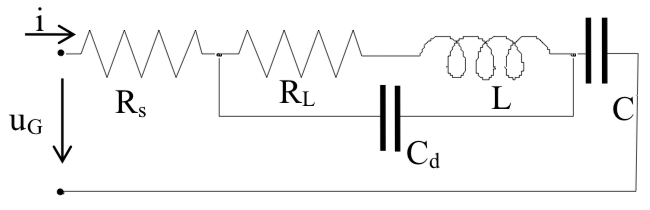
\includegraphics[width=0.6\linewidth]{circuito2.png}
			\caption{Circuito RLC tendo em conta a resistência e capacidade distribuídas na bobina}
			\label{fig:circuito2}
		\end{figure}
		\par
		Pela análise do circuito da figura \ref{fig:circuito2}, a expressão da impedância é dada por
		\begin{equation}
			\bar{Z} = \bar{Z}_{R_S} + \bar{Z}_{\parallel} + \bar{Z}_C,
		\end{equation}
		\par
		onde
		\begin{equation}
			\bar{Z}_{\parallel} = (\bar{Z}_{R_L} + \bar{Z}_{L}) \parallel \bar{Z}_{C_d} = \dfrac{\left(R_L + \mathrm{j} \omega L\right)\left(\dfrac{1}{\mathrm{j} \omega C_d}\right)}{(R_L + \mathrm{j} \omega L) + \dfrac{1}{\mathrm{j} \omega C_d}}, \hspace{2pt}\omega \neq 0.
		\end{equation}
		\par
		Supondo que $R_L \ll \omega L$, tem-se
		\begin{align*}
			\bar{Z} &= R_S + \dfrac{\left(R_L + \mathrm{j} \omega L\right)\left(\dfrac{1}{\mathrm{j} \omega C_d}\right)}{R_L + \mathrm{j} \omega L + \dfrac{1}{\mathrm{j} \omega C_d}} + \dfrac{1}{\mathrm{j} \omega C} \\
			&= R_S + \dfrac{1}{\mathrm{j} \omega C} + \dfrac{\left(\dfrac{R_L}{\omega L} + \mathrm{j}\right)\left(\dfrac{1}{\mathrm{j} \omega C_d}\right)}{\dfrac{R_L}{\omega L} + \mathrm{j} + \dfrac{1}{\mathrm{j} \omega^2 C_d L}} \\
			&\approx R_S + \dfrac{1}{\mathrm{j} \omega C} + \dfrac{\dfrac{1}{\omega C_d}}{\mathrm{j} + \dfrac{1}{\mathrm{j} \omega^2 C_d L}} \nonumber \\
			&= R_S + \dfrac{1}{\mathrm{j} \omega C} + -\mathrm{j}\dfrac{1}{\omega C_d - \dfrac{1}{\omega L}} \\
			&= \underbrace{R_S}_{=\Re{\bar{Z}}} + -\mathrm{j}\underbrace{\left(\dfrac{1}{\omega C} + \dfrac{1}{\omega C_d - \dfrac{1}{\omega L}}\right)}_{=\Im{\bar{Z}}}, \hspace{2pt}\omega \neq 0. \numberthis \\
		\end{align*}

		\par
		Na situação de ressonância do circuito, a corrente é máxima e encontra-se em fase com a tensão do gerador. Para que tal aconteça, é necessário que a impedância seja mínima e que
		\begin{equation}
			\Im{\bar{Z}} = \left(\dfrac{1}{\omega C} + \dfrac{1}{\omega C_d - \dfrac{1}{\omega L}}\right) = 0, \hspace{2pt}\omega \neq 0.
		\end{equation}

		\newpage
		Assim, tem-se
		\begin{align*}
			&\dfrac{1}{\omega C} + \dfrac{1}{\omega C_d - \dfrac{1}{\omega L}} = 0 \\
			&\Leftrightarrow \dfrac{1}{\omega C} = - \dfrac{1}{\omega C_d - \dfrac{1}{\omega L}} \\
			&\Leftrightarrow \omega C_d - \dfrac{1}{\omega L} = -\omega C \\
			&\Leftrightarrow \omega^2 C_d - \dfrac{1}{L} = -\omega^2 C \\
			&\Leftrightarrow \omega^2 \left(C + C_d \right) = \dfrac{1}{L} \\
			&\Leftrightarrow \omega^2 = \dfrac{1}{L\left(C + C_d \right)} \\
			&\Leftrightarrow \dfrac{1}{\omega^2} = L\left(C + C_d \right), \hspace{2pt}\omega \neq 0. \numberthis
		\end{align*}

	\subsection{}
		\begin{figure}[h]
			\centering
			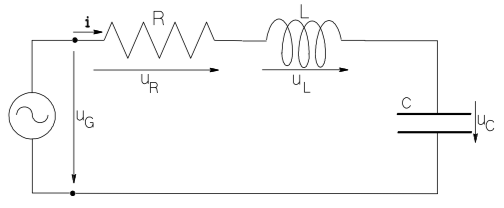
\includegraphics[width=0.6\linewidth]{circuito1.png}
			\caption{Circuito RLC série, $f_0 = \SI{40}{\kilo\hertz}, L = \SI{2,0}{\milli\henry}$ }
			\label{fig:circuito1}
		\end{figure}
		\par
		Pela análise do circuito da figura \ref{fig:circuito1}, no domínio do tempo, obtém-se
		\begin{equation*}
			u_G = u_R + u_L + u_C = Ri + L\dv{i}{t} + \dfrac{1}{C} \int{i\dd{t}}. \numberthis
		\end{equation*}
		\par
		Em amplitudes complexas, tem-se
		\begin{gather*}
			\bar{U}_G = \bar{U}_R + \bar{U}_L + \bar{U}_C = R\bar{I} + \mathrm{j} \omega L - \dfrac{\mathrm{j}}{\omega C}\bar{I} \numberthis \\
			\eq \dfrac{\bar{U}_G}{\bar{I}} = \bar{Z} = R + \mathrm{j}\left(\omega L - \dfrac{1}{\omega C}\right), \numberthis
		\end{gather*}

		onde

		\begin{align}
			Z &= \sqrt{R^2 + \left(\omega L - \dfrac{1}{\omega C}\right)^2} \\
			\alpha_Z &= \arctan{\left(\dfrac{\omega L - \dfrac{1}{\omega C}}{R}\right)}
		\end{align}

	\newpage
	\subsubsection{}
		\par
		Na situação de ressonância do circuito, $u_G$ e $i$ estão em fase.  Portanto, tal como visto anteriormente, a impedância é puramente resistiva, tendo então
		\begin{gather*}
			\Im{\bar{Z}} = \omega_0 L - \dfrac{1}{\omega_0 C} = 0 \\
			\eq \omega_0 L = \dfrac{1}{\omega_0 C}
		\end{gather*}
		\par
		De onde é possível obter o valor da capacidade $C$, dado por
		\begin{gather*}
			C = \dfrac{1}{\omega_0^2 L} = \dfrac{1}{\left(2\pi \times \num{40e3}\right)^2 \times \num{2e-3}} \approx \SI{7.916}{\nano\farad}
		\end{gather*}

	\subsubsection{}
		\par
		A expressão da corrente normalizada $I_n$ em função da frequência normalizada $f_n$ é dada por

		\begin{align}
			\label{In(fn)}
			I _ { n } \left( f _ { n } \right) = \frac { 1} { \sqrt { 1+ Q _ { 0} ^ { 2} \left( f _ { n } - 1/ f _ { n } \right) ^ { 2} } }
		\end{align}

		onde $ f _ { n } = f / f _ { 0} \hspace{4pt}\text{e}\hspace{4pt}  Q _ { 0} = \left( \omega _ { 0} L / R _ { S } \right)$.
		Para $R_S = 250\hspace{4pt}\Omega$ e para $R_S = 500\hspace{4pt}\Omega$, substituindo em \ref{In(fn)}, tem-se

		\begin{align}
			\label{In_250}
			I _ { n } \left( f _ { n } \right) = \frac {1} {  \sqrt { 1+ \left(\frac{2\pi \times \num{40e3} \times \num{2e-3}}{250} \right)^{2}  \left( f _ { n } - 1/ f _ { n } \right) ^ { 2} }}
		\end{align}

		\begin{align}
			\label{In_500}
			I _ { n } \left( f _ { n } \right) = \frac {1} {  \sqrt { 1+ \left(\frac{2\pi \times \num{40e3} \times \num{2e-3}}{500} \right)^{2}   \left( f _ { n } - 1/ f _ { n } \right) ^ { 2} }}, \\
		\end{align}

	respetivamente. As duas curvas correspondentes a (\ref{In_250}) e (\ref{In_500}) foram obtidas recorrendo ao Matlab e estão representadas em anexo na secção R 3.2 b).


	\subsubsection{}

		Recorrendo a (8), obtém-se as expressões da corrente $i$ e das tensões no condensador, na bobina e na resistência, $u_C$, $u_L$, e $u_R$ respetivamente, dadas por

		\begin{align*}
			\bar{U}_G = \bar{Z} \bar{I} \eq \bar{I} = \dfrac{\bar{U}_G}{\bar{Z}} & \eq I_{ef} \mathrm{e}^{\mathrm{j} \alpha_I} = \dfrac{U_{G_{ef}}}{Z} \mathrm{e}^{\mathrm{j}\left(\alpha_{U_G} - \alpha_{Z}\right)}\\
			\bar{U}_C = -\mathrm{j} \dfrac{1}{\omega C} \bar{I} &\eq U_{C_{ef}} \mathrm{e}^{\mathrm{j} \alpha_{U_C}}= \dfrac{1}{\omega C}I_{ef} \mathrm{e}^{\mathrm{j} \left(-\frac{\pi}{2}+\alpha_I\right)} \\
			\bar{U}_L = \mathrm{j}\omega L \bar{I} &\eq U_{L_{ef}} \mathrm{e}^{\mathrm{j} \alpha_{U_C}}=\omega LI_{ef} \mathrm{e}^{\mathrm{j} \left(\frac{\pi}{2}+\alpha_I\right)}  \\
			\bar{U}_R = R \bar{I} &\eq {U}_{R_{ef}}\mathrm{e}^{\mathrm{j} \alpha_R}= R I_{ef} \mathrm{e}^{\mathrm{j} \alpha_I}.\\
		\end{align*}

		Considerando os seguintes dados

		\begin{align*}
			&R _ { s } = 250\hspace{4pt}\Omega \\
			&U_{G_{ef}} = 1\hspace{2pt}V\\
			&C \approx \SI{7.916}{\nano\farad}\\
			&L = \SI{2}{\milli\farad}, \\
		\end{align*}

		 obtém-se, para as frequências $f = f_0 = \SI{40}{\kilo\hertz}$, $f_1 = 0.95f_0= \SI{38}{\kilo\hertz}$ $f_2 = 1.05f_0 = \SI{42}{\kilo\hertz}$, os valores eficazes e desfasagens corrente e das tensões no condensador, na bobina e na resistência, apresentados em anexo na tabela da secção R 3.2 c).

	\newpage
	\subsubsection{}

		Na figura \ref{fig:diag_vect}, estão representados os diagramas vetoriais de tensão para cada uma das frequência da alínea anterior.

		\begin{figure}[h]
			\centering
			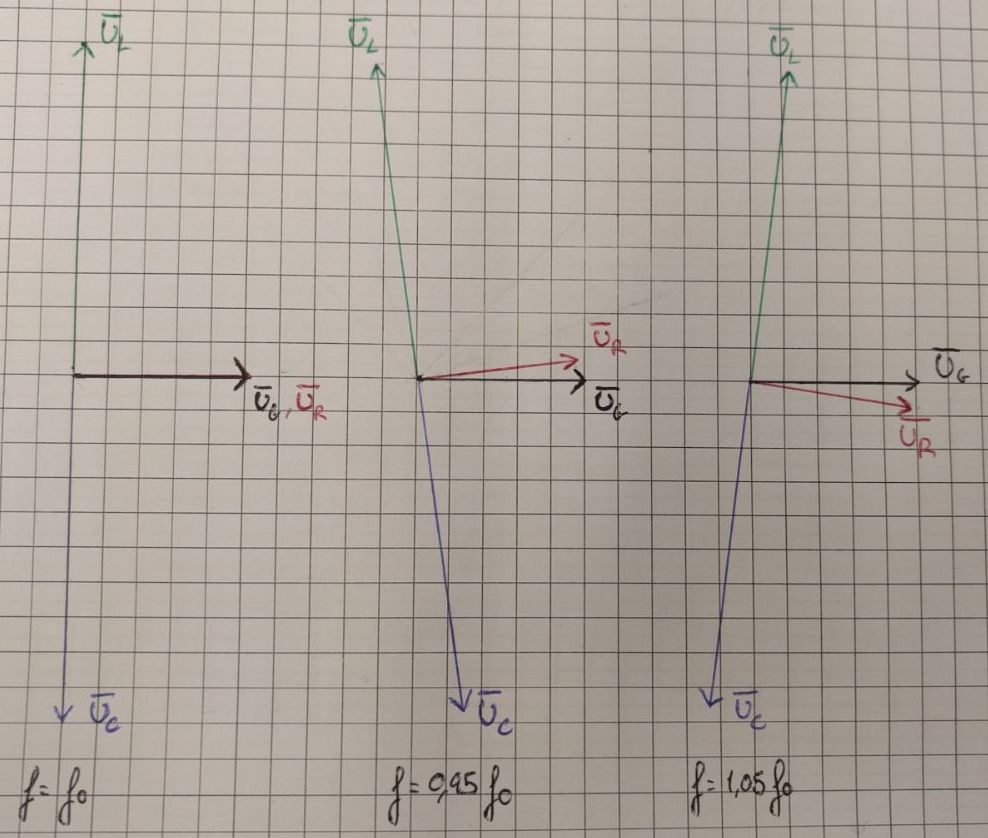
\includegraphics[width=0.6\linewidth]{diag_vect.jpeg}
			\caption{Diagrama vetorial das tensões do circuito RLC para $f=f_0$, $f_1=0.95f_0$ e $f_2=1.05f_0$, respetivamente.}
			\label{fig:diag_vect}
		\end{figure}

	%Ver \autoref{fig:figure-example}

	%\printbibliography

\end{document}
